\begin{center}


\tikzset{every picture/.style={line width=0.75pt}} %set default line width to 0.75pt        

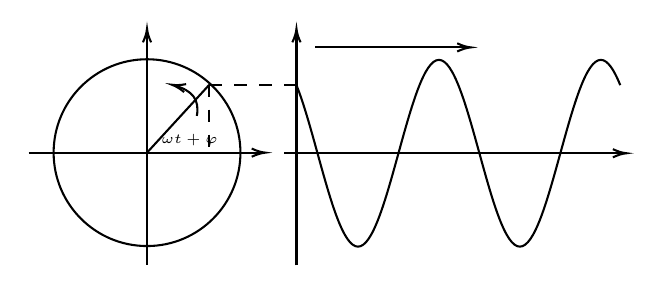
\begin{tikzpicture}[x=0.75pt,y=0.75pt,yscale=-0.6,xscale=0.6]
%uncomment if require: \path (0,300); %set diagram left start at 0, and has height of 300

%Straight Lines [id:da6372713083546984] 
\draw    (65,169.52) -- (253,169.52) ;
\draw [shift={(255,169.52)}, rotate = 180] [color={rgb, 255:red, 0; green, 0; blue, 0 }  ][line width=0.75]    (10.93,-3.29) .. controls (6.95,-1.4) and (3.31,-0.3) .. (0,0) .. controls (3.31,0.3) and (6.95,1.4) .. (10.93,3.29)   ;
%Straight Lines [id:da44936558403337346] 
\draw    (160,72) -- (160,260) ;
\draw [shift={(160,70)}, rotate = 90] [color={rgb, 255:red, 0; green, 0; blue, 0 }  ][line width=0.75]    (10.93,-3.29) .. controls (6.95,-1.4) and (3.31,-0.3) .. (0,0) .. controls (3.31,0.3) and (6.95,1.4) .. (10.93,3.29)   ;
%Shape: Circle [id:dp23986433167584287] 
\draw   (85,169.52) .. controls (85,128.1) and (118.58,94.52) .. (160,94.52) .. controls (201.42,94.52) and (235,128.1) .. (235,169.52) .. controls (235,210.95) and (201.42,244.52) .. (160,244.52) .. controls (118.58,244.52) and (85,210.95) .. (85,169.52) -- cycle ;
%Straight Lines [id:da671297841722321] 
\draw    (210,115) -- (160,169.52) ;
%Straight Lines [id:da5109888412647536] 
\draw  [dash pattern={on 4.5pt off 4.5pt}]  (210,115) -- (210,170) ;
%Straight Lines [id:da0436893772008915] 
\draw    (270,170) -- (543,170) ;
\draw [shift={(545,170)}, rotate = 180] [color={rgb, 255:red, 0; green, 0; blue, 0 }  ][line width=0.75]    (10.93,-3.29) .. controls (6.95,-1.4) and (3.31,-0.3) .. (0,0) .. controls (3.31,0.3) and (6.95,1.4) .. (10.93,3.29)   ;
%Shape: Wave [id:dp7780237593069468] 
\draw   (280,115.32) .. controls (285.71,129.5) and (291.24,149.49) .. (296.9,170) .. controls (307.5,208.42) and (317.64,245) .. (329.4,245) .. controls (341.16,245) and (351.3,208.42) .. (361.9,170) .. controls (372.5,131.58) and (382.64,95) .. (394.4,95) .. controls (406.16,95) and (416.3,131.58) .. (426.9,170) .. controls (437.5,208.42) and (447.64,245) .. (459.4,245) .. controls (471.16,245) and (481.3,208.42) .. (491.9,170) .. controls (502.5,131.58) and (512.64,95) .. (524.4,95) .. controls (529.88,95) and (535.01,102.95) .. (540,115.32) ;
%Straight Lines [id:da6835536982366524] 
\draw  [dash pattern={on 4.5pt off 4.5pt}]  (210,115) -- (280,115) ;
%Straight Lines [id:da9401330418494154] 
\draw    (280,260) -- (280,72) ;
\draw [shift={(280,70)}, rotate = 90] [color={rgb, 255:red, 0; green, 0; blue, 0 }  ][line width=0.75]    (10.93,-3.29) .. controls (6.95,-1.4) and (3.31,-0.3) .. (0,0) .. controls (3.31,0.3) and (6.95,1.4) .. (10.93,3.29)   ;
%Straight Lines [id:da5155994625073528] 
\draw    (295,85) -- (418,85) ;
\draw [shift={(420,85)}, rotate = 180] [color={rgb, 255:red, 0; green, 0; blue, 0 }  ][line width=0.75]    (10.93,-3.29) .. controls (6.95,-1.4) and (3.31,-0.3) .. (0,0) .. controls (3.31,0.3) and (6.95,1.4) .. (10.93,3.29)   ;
%Curve Lines [id:da19556548359672776] 
\draw    (200,140) .. controls (202.24,127.01) and (196.8,119.73) .. (181.91,115.51) ;
\draw [shift={(180,115)}, rotate = 14.19] [color={rgb, 255:red, 0; green, 0; blue, 0 }  ][line width=0.75]    (10.93,-3.29) .. controls (6.95,-1.4) and (3.31,-0.3) .. (0,0) .. controls (3.31,0.3) and (6.95,1.4) .. (10.93,3.29)   ;

% Text Node
\draw (169,152.4) node [anchor=north west][inner sep=0.75pt]  [font=\tiny]  {$\omega t+\varphi $};


\end{tikzpicture}

\end{center}